\documentclass[]{article}

%opening
\title{FYS-STK 4155 Project 3}
\author{Zakarias L. Hejlesen}
\usepackage[hidelinks]{hyperref}
\usepackage{todonotes}
\usepackage{amsmath}
\usepackage{graphicx}
\usepackage{bm}
\usepackage{algorithmic}
\usepackage{listings}
%\usepackage{minted}
\usepackage{xcolor}
\usepackage{amsfonts}
\usepackage{array,multirow,graphicx}
\usepackage{float}
\usepackage[boxed, noline]{algorithm2e}

\lstloadlanguages{Python}
\lstset{
	language=Python,
	basicstyle=\scriptsize\sffamily,
	numberstyle=\color{gray},
	stringstyle=\color[HTML]{933797},
	commentstyle=\color[HTML]{228B22}\sffamily,
	emph={[2]from,import,pass,return}, emphstyle={[2]\color[HTML]{DD52F0}},
	emph={[3]range}, emphstyle={[3]\color[HTML]{D17032}},
	emph={[4]for,in,def}, emphstyle={[4]\color{blue}},
	showstringspaces=false,
	breaklines=true,
	prebreak=\mbox{{\color{gray}\tiny$\searrow$}},
	numbers=left,
	xleftmargin=15pt
}

% To move algorithm2e caption a bit below the box
\SetAlCapSkip{1em}

\begin{document}

\maketitle

\begin{abstract}
	In this project we aim to determine the critical temperature $T_\text{KT}$ for the Kosterlitz-Thouless phase transition in the planar XY model using regular and convolutional neural nets. We generate the datasets ourselves; though they exhibit the expected phase transition they are of too poor quality to predict the critical temperature on the infinite plane. We find that convolutional nets are significantly better than regular nets at classifying states as being above or below the critical temperature when trained on small datasets. On larger datasets both types of nets become extremely accurate(0.97 and above) and our best variants yield predictions for the critical temperature that equal that obtained from Monte-Carlo simulations to a deviation less than $10^{-16}$. All code and plots relevant to the project may be found at \url{https://github.com/ethq/FYSSTK-Project3}.
\end{abstract}

\section{Introduction}
In this project we aim to determine the critical temperature $T_\text{KT}$ for the phase transition in the two dimensional XY model, using regular neural nets(NNs) and various convolutional neural nets(CNNs). To do so, we will first generate our own datasets through Markov-Chain Monte-Carlo sampling, aiming at least for a uniform distribution of states over a temperature interval containing $T_\text{KT}$.\footnote{Though we unfortunately do not sample the microcanonical ensemble directly. It is not clear at this point how this will affect my results.} We label each state with the temperature of the system it was drawn from, as thermal fluctuations render the energy an inaccurate measure for classification. We expect the CNN will outperform the NN as it can explicitly make use of 2D information in the state.

We are also interested in the effect of feature engineering. In particular, we know that the transition in the XY-model is a vortex-unbinding transition(more on this shortly). As such we expect the vorticity to be a good measure for classification. The question is then: if we convert a raw spin configuration to a vorticity configuration, will the (C)NNs perform better or worse?

Having read about residual nets, we also attempt to train one of these on our states. Our initial hope is that they can yield even better performance than our other nets, owing to their extremely high accuracy in ML competitions.

The inspiration for this project is ref. \cite{PhysRevB.97.045207}, the main topic of which is whether neural nets can learn $T_\text{KT}$ in the XY-model. I hope to apply what I learn to my own research, in particular whether it is possible for a neural net to learn a particular transition temperature in quantum vortex matter.\footnote{To be more specific, the transition in question is the Onsager transition\cite{onsager} to clustered, negative temperature states for vortex matter in superfluids, which might consist of e.g. Helium or Rubidium. It has been experimentally observed quite recently.\cite{Gauthier1264} Incidentally, the order parameter is exactly the same as it is in the planar XY model.}

\section{Formalism}
Let us briefly introduce the XY model. It is governed by the Hamiltonian
\begin{align}
H = -J\sum_{\langle ij\rangle}s_i\cdot s_j = -J\sum_{\langle ij\rangle}\cos(\theta_i-\theta_j)
\end{align}
where $\langle ij \rangle$ indicates nearest-neighbour summation and $s_i$ denotes a planar unit spin at lattice site $i$. This model exhibits some remarkable properties - in particular a phase transition. This is surprising in the context of the Mermin-Wagner theorem\cite{PhysRevLett.17.1133}, which states that continuous symmetries cannot be broken in two dimensions. However, phase transitions need not be associated with symmetry breaking, and indeed the phase transition in the XY-model is one such example. Instead it is an example of a Kosterlitz-Thouless(KT) transition, and it is characterized by the behaviour of vortices.\footnote{Sometimes also referred to as a topological phase transition, where the vortices are the topological defects. They are so named because 1) they are "topologically protected" - immune to local perturbations and 2) yield a singularity in the order parameter field. Topological protection arises because single defect states are not homotopic to smooth states(though a vortex-antivortex state is), and forcibly changing the topology has a high energy cost.} Vortices are rotational structures in the spin; if we sum up the spins around a loop enclosing a vortex it must be an integer multiple of $2\pi$. The integer multiplying $2\pi$ is usually referred to as the vortex charge.

Below the transition temperature $T = T_\text{KT}$, vortices and anti-vortices are tightly bound in pairs. This means they influence the surrounding spin field only locally, and so one finds that the spin correlation function decays algebraically in this regime. However, at $T > T_\text{KT}$, it becomes energetically favourable for the vortices to unbind. The free or quasi-free vortices then influence the spin field in a chaotic manner, and this leads to an exponential decay in the spin correlation function. Hence the system goes from a state with quasi long-range order to an unordered state - a phase transition. The exact value of $T_\text{KT}$ on an infinite lattice can be found through Monte-Carlo simulations, and has been determined to be $T_\text{KT}^\infty = 0.893 \pm 0.002$.\cite{Olsson_1991}

\subsection{Convolutional neural nets}
As we will see, our regular neural net does not do spectacularly well when it comes to classifing the states of the XY model. The hope is that we can improve our result by using a \textit{convolutional} neural net(CNN) instead. These offer several advantages over regular neural nets, especially when it comes to computer vision. For example:

\begin{itemize}
	\item[1)] There are less weights to train. CNNs are tailored to image analysis and make use of the fact that pixel data is often highly locally correlated. 
	
	\item[2)] Global feature recognition. While a NN learning to recognize a rabbit in the lower left corner of an image will not be able to recognize a rabbit in the top right, a CNN can.
\end{itemize}

In terms of architecture, CNNs differ from regular NNs in that they include different types of layers. Commonly, a CNN will contain:
\begin{itemize}
	\item[1)] \textbf{A convolutional layer.} This is the backbone of the CNN. The layer has $N$ associated \textit{filters}, which act as the neurons. Each filter is a matrix of dimension\footnote{This dimension is referred to as the receptive field, as it describes how much of the image a filter will see.} $l_x\times l_y$ and is convolved with the preceding input layer to produce the output. Filters act as feature extractors and are thus responsible for CNNs being able to apply knowledge learned in one part of the image to another part of the image. As an example, we mention the famous Sobel filter which is mainly used for edge detection.  Typically the input layer is padded with zeros to ensure that the convolutional layer does not reduce the spatial dimensions of the data. This is advantageous when it comes to preserving information at the edges, and is mandatory in more advanced architectures(e.g. residual nets) where a constant spatial dimension is demanded. Choosing the number of filters in a layer is a black art, but we note that performance saturates when we have one filter centered at each pixel(including padding). Consequently there is no point in having more than 81 filters to process a 7x7 image, for example. Another rule of thumb is to increase the number of filters in consecutive layers. In this way the lowest layers learn the coarsest features, and later layers can then combine them to resolve finer details.
	\item[2)] \textbf{An activation layer.} As always, we need to introduce some kind of non-linearity for our net to be a universal function approximator. We usually apply one after each convolutional layer to increase the level of feature extraction; if we simply stack two convolution layers on top then the second will act only on a linear transformation of the first input, which may not yield a significant advantage over just a single layer. 
	\item[3)] \textbf{A pooling layer.} Similar to a convolutional layer, except now the filter is replaced with either a max or average operation. Acts as regularization and downsamples the image. Typically used after several convolutional layers have been applied. 
	\item[4)] \textbf{A dropout layer.} Also a type of regularization, familiar from NNs. Randomly kills off a fraction of neurons/filters during training(though only for one pass, after which they are revived). Also causes the net to become more robust; if a filter has learned to recognize flying turtles and is then killed, other filters have to step in and learn how to recognize flying turtles too. Using nets with dropout layers is in a sense similar to ensembling nets; effectively dropout causes "multiple" nets to be simultaneously trained and averaged.\cite{Hinton2012ImprovingNN}
	\item[4]) \textbf{A dense layer.} These are just the fully connected layers used in regular NNs. Typically some of these are used as the last layers in a CNN. The first of these consist of a relatively high number of neurons and learns global features, whereas the last is the output layer and has a number of neurons equal to the number of classes.
\end{itemize}

\subsection{Residual nets}
Deep nets suffered for a long time from the problem of vanishing/exploding gradients - that weights will either vanish or blow up by repeated multiplication through a large number of layers. Although this problem is now typically dealt with by both normalized weight initialization and the introduction of normalization layers\cite{LeCun2012}, it was found that even so, deep nets attain a maximal accuracy which then subsequently begins to degrade.\cite{degrad} Incidentally, this loss of accuracy - which also affects the trainng data - has nothing to do with overfitting. This degradation problem was the motivation for the introduction of so-called residual nets, or ResNets.\cite{resnet}

The key insight of the creators of the ResNet architecture was that identity mappings are not easy for multiple non-linear layers to approximate. Indeed, experiments show that if one simply inserts several layers performing an identity mapping into a given architecture, performance degrades. 

To resolve the problem, let us first consider a stack of layers whose job is to produce an approximation of a map $\mathcal{H}(x)$ capable of yielding perfect predictions. Now, if $\mathcal{H}$ is very close to the identity map, degradation is likely to occur. Hence the authors hypothesized that one may obtain better predictions by instead trying to approximate $\mathcal{F}(x) \equiv \mathcal{H}(x) - x$.\footnote{This is why ResNets need input/output dimensions to be equal.} After our non-linear layers have approximated $\mathcal{F}(x)$, we then simply add in $x$ to obtain an approximation of $\mathcal{H}(x)$. In total, these operations comprise a \textit{residual block}, as shown in Fig. \ref{fig:residual_block}.

\begin{figure}
	\centering
	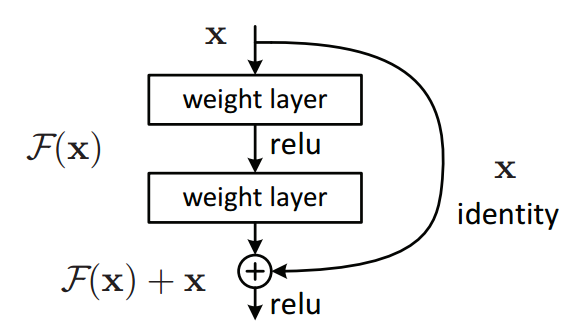
\includegraphics[width=200px]{residual_block.png}
	\caption{A residual block, figure taken from ref. \cite{resnet}}
	\label{fig:residual_block}
\end{figure}

A regular deep net can then be converted to a residual net by simply replacing stacks of convolutional layers by residual blocks. This turns out to work so well that the authors obtained first place in the 2015 ILSVRC classification competition, using an ensemble consisting of six 152-layer residual nets. 

\subsection{Transfer learning}
When using ResNets or any other state of the art CNN, one might also want to utilize the weights learned on e.g. ImageNet. Incidentally, this training process can take weeks, and for this reason one can download pre-trained models for direct use. In Keras, several such models(VGG, ResNets, DenseNets, Inceptions etc.) are included in the applications module. A given project will typically not have the same number of classes as ImageNet(some 20 000 in number), so what one does is to strip off the classification layer and insert a new one with the appropriate number of neurons. For added flexibility, one may also allow a number of lower layers to be trained. Other than that, the weights from the remaining layers are simply transferred and used as-is. 

\section{Methods}

\subsection{Data generation}
Our desired dataset consists of a set of sample states of the XY model on a square lattice of dimension $L$, each at fixed energy and temperature. As these are one to one only in the thermodynamic limit, our representative states at fixed temperature $T$ will have fluctuating and differing energies $E_i$. Sampling the microcanonical ensemble directly quickly becomes unfeasible, and so we resort to sampling using a Markov-Chain Monte-Carlo(MCMC) method - the Metropolis algorithm. To generate a state at temperature T, we start with a uniformly distributed spin configuration. We then run the Metropolis algorithm(shown below) until successive energy values are within a specified tolerance, at which point we assume equilibrium has been reached. For calculating expectation values - energy in particular - we then proceed to sample the state space $M$ times, each separated by $N$ Metropolis steps to minimize autocorrelations in the states. Statistical quantities are then obtained by averaging over our samples. In what follows, we will refer to particular datasets with the notation $(L,M,N)$ where needed.

\begin{algorithm}
	\caption{The Metropolis algorithm. Above we illustrate a full sweep, e.g. an MCMC step applied to each spin in the system.}
	
	T = get\_temperature()\\
	set\_initial\_config()\\

	\For{\text{s in spins}}{
		$E_0$ = compute\_energy()\\
		flip\_spin(s)\\
		$E_1$ = compute\_energy()\\
		$\Delta E$ = $E_1 - E_0$\\
		\textit{r} = uniform\_random()\\
		\If{\text{r} $ < \exp\left(-\Delta E/T\right)$}{
			Update current state\\
		}
	}
\end{algorithm} 
\vspace{5px}

\subsection{Locating $T_\text{KT}$ from neural net predictions}
When we train our nets, we feed them either a raw spin configuration or a vortex configuration. Though they can learn the energy of a state from such a configuration, it does - as mentioned - not uniquely identify the temperature. Hence our nets will need to learn other features of a state in order to correctly classify it as being above or below $T_\text{KT}$, such as vorticity or magnetization. 

Nonetheless, whatever the network does learn, we must subsequently infer $T_\text{KT}$ from its predictions. Firstly, states at or close to the critical temperature should be the ones that are most difficult to classify. Hence we need to look at the states for which our network outputs a probability of $\approx .5$. Again, the temperature of these states is unknown to us, but we can compute their mean energy. Using OLS on the mean energies computed at all temperatures, we can then infer a temperature from any given mean energy. And this finally leads us to the critical temperature predicted by our nets. To streamline the process, we have done this by first plotting class prediction probabilities as a function of energy. To quickly compute the mean, we fit a fifth order polynomial to the predictions. Their point of intersection corresponds to probability $p = .5$, and using our abovementioned "table" we convert the corresponding mean energy to the predicted $T_\text{KT}$. For visualization, see Fig. \ref{fig:energy_heatcap_example}R in the Results section.

\subsection{Spin- to vortex-configuration conversion}
The states we generate are explicitly spin configurations; at each lattice point $x_{ij}$ there is a planar spin $\theta_{ij}$. From it, we can easily extract the vorticity. We will assume that our system has only singly-charged vorticies, e.g. any closed loop $\partial\Sigma$ containing a vortex implies a phase change of $2\pi$: $\int_{\partial\Sigma} \theta = 2\pi$. Consider a 2x2 square containing a vortex, with the following spin values:
\begin{align}
\theta_{ij} = \begin{pmatrix} 0 & 2\pi \\ \pi/2 & \pi/2\end{pmatrix}
\end{align}
Looping around the square counterclockwise from the top left, we can calculate the angle differences:
\begin{align}
\Delta\theta_{ij} = \begin{pmatrix}
-2\pi & \pi\\ \pi/2 & \pi/2
\end{pmatrix}
\end{align}
Note that summing all angle differences simply yields zero - as it must. However, we can explicitly remove phase changes of $\pm\ 2\pi$ to identify vortices by applying the sawtooth function:
\begin{align}
\text{saw}(x) = \begin{cases} 
x+2\pi, & x < -\pi \\
x, & -\pi \leq x \leq \pi \\
x-2\pi, & \pi < x
\end{cases}
\end{align}
Applying the saw function to the spin differences above and then summing, we are left with $2\pi$ - identifying a vortex. On the other hand, if there is \textit{no} vortex, then $\Delta \theta_{ij} \in [-\pi, \pi]$ and $\sum_{\partial\Sigma}\text{saw}(\Delta\theta_{ij}) = 0$. Consequently the vortex representation is typically very sparse. After normalization, the configuration will contain mostly zeroes and a few ones here and there where a vortex lives.

\subsubsection{Resampling and scoring}
For scoring our classifiers, we typically use the accuracy, which is computed as
\begin{align}
\text{Accuracy} = \frac{tp+tn}{tp+tn+fp+fn}
\end{align}
Where we have used standard notation, e.g. $tp = \text{true positives}, fn = \text{false negatives}$ and so on. This is usually a good metric to use, except when the dataset is imbalanced and in which case it may be exceptionally \textit{bad}. It may then be more informative to look at something like the F1-score, defined as
\begin{align}
\text{F}1 = 2\frac{\text{precision}\cdot\text{recall}}{\text{precision}+\text{recall}}
\end{align}
where
\begin{align}
\text{precision} = \frac{tp}{tp+fp} && \text{recall} = \frac{tp}{tp+fn}
\end{align}
As opposed to the accuracy, the F1-score \textit{is} sensitive to misclassifications. Just as accuracy, the best possible F1 score is unity and the worst is zero. Note that for binary classification, these and several other scores depend only on $tp, tn, fp$ and $fn$, which are usually put in the so-called confusion matrix. To quickly assess the performance our models, we have saved these to Plots/Confusion Matrix/.\footnote{Note that an error in my code caused the (7, 500, 5) plots to look as if there are ~90\% misclassifications. This of course isn't true; the labels on the plot should be switched around.}

Some of our datasets have imbalanced class ratios, and this \textit{may} result in our classifiers simply learning to output the majority class(regardless of input) and in that way obtaining a fairly good accuracy. To see whether this is the case, one may use the aforementioned F1-score, look at the confusion matrix or similar. Nonetheless, if the problem is there we need to take care of it. Many methods exist: we may under/oversample, weight the cost function differently for minority and majority classes, synthesize new training instances in the minority class and so on. 

In undersampling, a number of training instances from the majority class equaling the number of training instances from the minority class is selected at random. For oversampling, one re-samples training instances from the minority class at random until equality is reached. Both of these methods have drawbacks: undersampling discards a lot of data, and though we may expect less misclassifications the accuracy is likely to decrease. Oversampling on the other hand introduces unwanted bias into the data by effectively weighting the resampled instances higher than the rest. Synthesizing new training instances avoids both these drawbacks, but as we will see introduces others. In this project we use the SMOTE algorithm to synthesize new data. Very roughly it creates an instance by taking linear combinations of old ones, with randomly varying weights.

\section{Results}
We begin by reporting on the quality of our generated datasets. It's a mixed bag - while all datasets generate energy and heat capacity curves(see Fig. \ref{fig:energy_heatcap_example}) with the qualitative features we expect, we can determine that the statistical averages cannot be exactly correct. To do so, we refer to the fact that one may determine the scaling of $T_\text{KT}$ with lattice dimension $L$ with the help of renormalization group techniques. In particular, the scaling is given by\cite{PhysRevLett.39.1201}
\begin{align}
T_\text{KT}^L = T_\text{KT}^\infty + c\frac{1}{(\log L)^2}
\end{align}
where $c$ is a positive constant. For a small number of measurements we do not observe scaling with $c > 0$, though increasing the number of measurements fixes this issue as shown in Fig. \ref{fig:tkt_scaling_L}. Unfortunately the predicted transition temperature on the infinite lattice is off in both cases. Nonetheless, each dataset \textit{does} have a well-defined transition temperature, as may be observed by the maximum in the heat capacity. And we can still see whether our neural nets can learn this particular point if we feed them either the spin or vortex configuration.

\begin{figure}[H]
	\vspace{-10px}
	\centering
	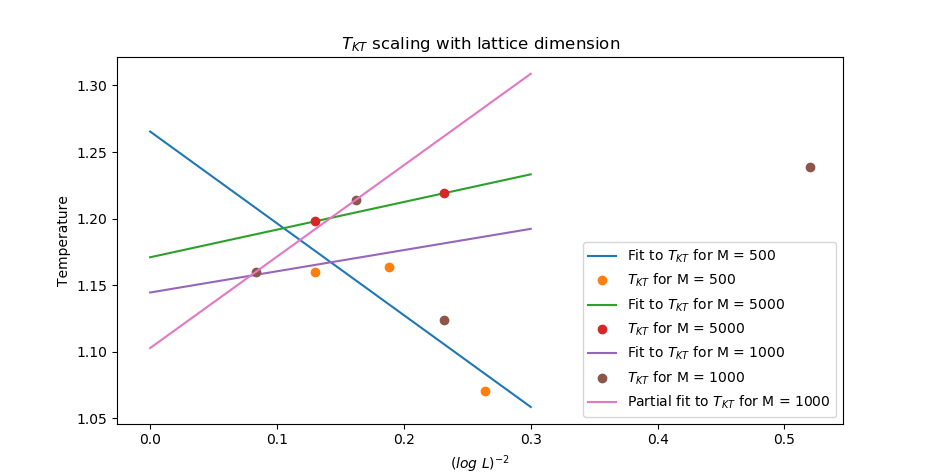
\includegraphics[width=280px]{../Plots/Tkt_scaling_with_lattice_2.png}
	\caption{Scaling of $T_\text{KT}$ as inferred by the maximum of the heat capacity measured on different lattice sizes. For $M = 500$ measurements, the scaling is clearly wrong. For this reason we haven't bothered to plot any more datapoints. For $M = 5000$ measurements, the computational cost is extremely heavy(on my machine, it took three full days to generate (16, 5000, 1) for example). For this reason, we have but two datapoints. Of some comfort is that the slope now has the correct sign. The value of $T_\text{KT}^\infty$ - inferred from the intercept - is 1.27, 1.17 and 1.14 respectively, all off from the true value of 0.89. Note that the measurements on small lattices are more noisy than those on large lattices, as expected. Disregarding the datapoints from L = 4 and L = 8, the $M = 1000$ measurements yield an intercept of $T_\text{KT}^\infty = 1.10$. Visually it seems that the fit is rotated counter-clockwise as measurements are increased; we believe correct results will be obtained by increasing the number of measurements and/or time allowed to relax to equilibrium. }
	\label{fig:tkt_scaling_L}
\end{figure}

\begin{figure}
	\hspace{-40px}
	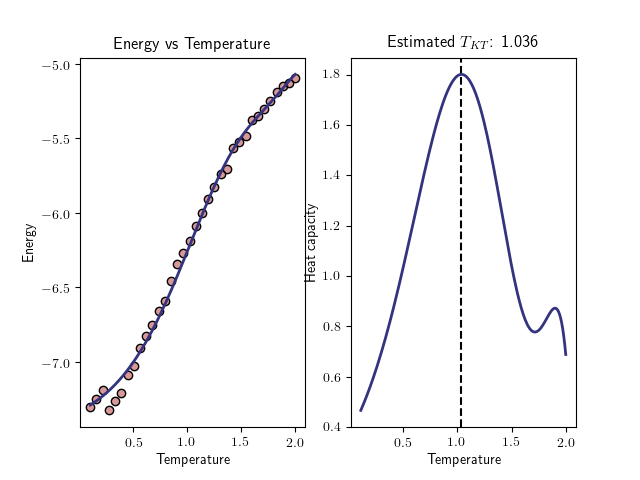
\includegraphics[width=200px]{../Plots/Predictions/MCMC_V0_L7_M500_N5.png}
	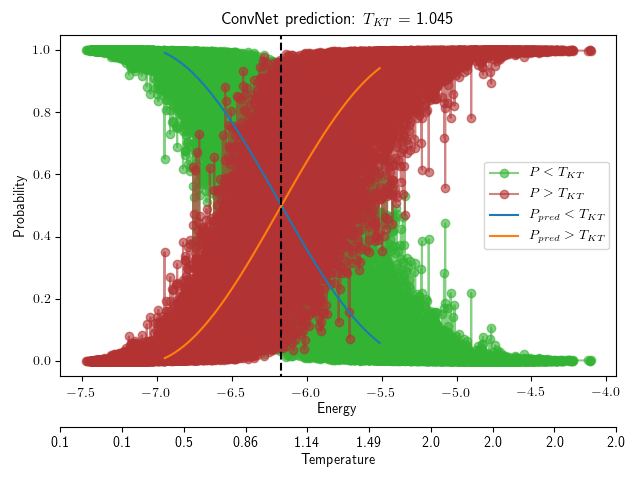
\includegraphics[width=200px]{../Plots/Predictions/CNN_V0_L7_M500_N5_2xConvConvPoolDrop.png}
	\caption{Dataset used: (7, 500, 5). \textbf{Left:} Energy and heat capacity as function of temperature. We plot only every third datapoint for clarity. We interpolate the curves with 10th order polynomials, which slightly overfits and yields the odd edge effects. $T_\text{KT}$ is inferred from the maximum of the heat capacity. The lack of a discontinuity signifies that it is a phase transition of infinite order. \textbf{Right:} Convolutional network prediction of $T_\text{KT}$, trained on raw spin configuration. Architecture used: 3xConv2xDropDense(see Plots/Model Graphs/ on GitHub). We assume that a rough decision boundary can be plotted as a function of energy. As the ConvNet does not have access to temperature information, we instead plot probabilities versus energy and average, as $\langle E \rangle \leftrightarrow T$ should be 1-1 in the limit of infinite measurements. We then identify the critical temperature with the point where the ConvNet is most uncertain about how to classify a state.}
	\label{fig:energy_heatcap_example}
\end{figure}

\subsection{Neural nets}
Let us now look at how regular neural nets do when it comes to predicting $T_\text{KT}$. We present here the analysis for (7, 500, 5), due to computational time saved. 

As in the last project, we do a gridsearch over learning type, learning rate, number of neurons in hidden layers and number of hidden layers. We do this for (7, 500, 5), and assume the results remain valid when we scale up to e.g. L = 16, though this of course needs to be checked. We find that a constant learning rate is better than an adaptive, and two hidden layers seem to be optimal, at least for the learning rates we have explored. A deeper network could very well be used, but then we need to combat vanishing gradients in some way. As for $L_2$-regularization, we find only gains of order $10^{-3}$ in the accuracy as we vary the parameter. Looking at the training history, we see that this is to be expected as we are typically not overfitting until the very last epochs. The results for neuron number/learning rate are shown in Fig. \ref{fig:neuralnet_75005_gsv}(after the bibliography). We note that this gridsearch was done using sklearn's MLPClassifier; some of our nets are trained using Keras with the AdaDelta optimizer, which uses an adaptive learning rate. 

\begin{figure}[h]
	\hspace{-120px}
	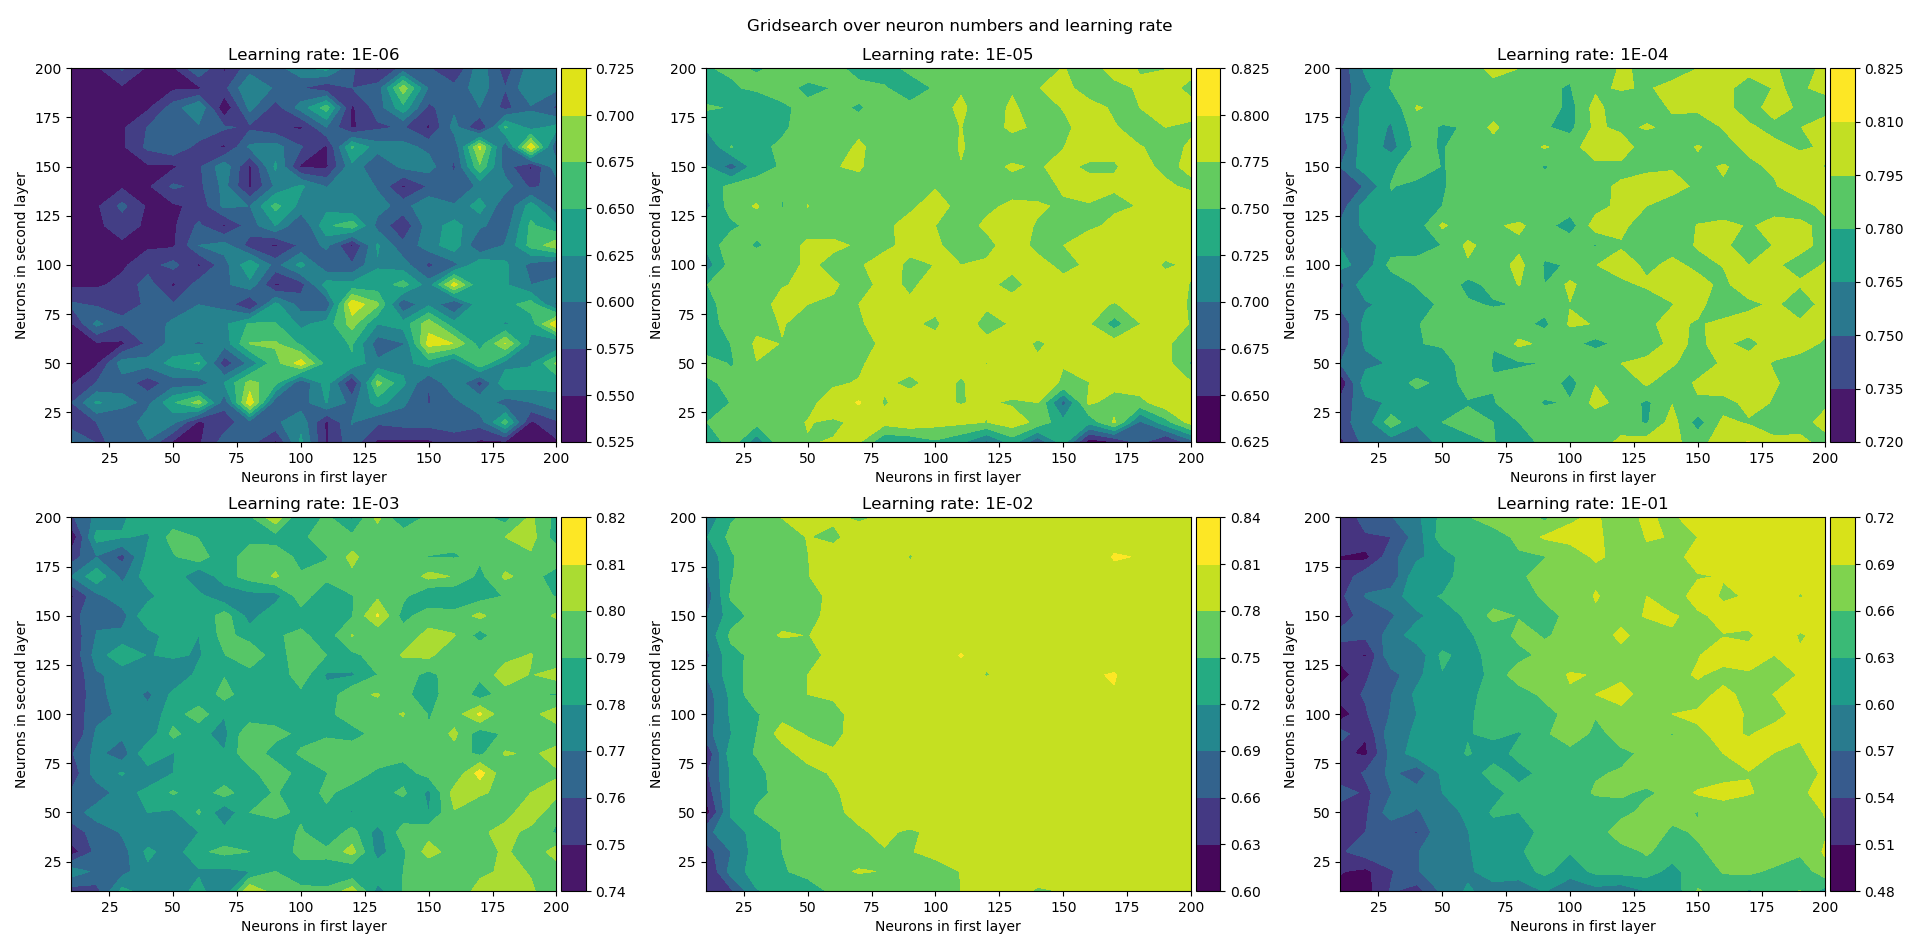
\includegraphics[width=600px]{../Plots/nn_gridsearch_neurons_lr.png}
	\label{fig:neuralnet_75005_gsv}
	\caption{Gridsearch over neuron number/learning rate. We see that for high learning rates, the high scores are concentrated in the upper right corner, e.g. both hidden layers have a high number of neurons. This seems not to be true as the learning rate decreases, e.g. lower number of hidden neurons in the second hidden layer seems advantageous. This should just be due to non-convergence - if the gridsearch had been run for some more epochs, I believe the same pattern would emerge: more neurons is simply better - as long as we don't overfit.}
\end{figure}

From the gridsearch we conclude that increasing neuron number seems to always yield better scores, assuming convergence. To make sure, we train three slightly different nets using Keras: 
\begin{itemize}
	\item[1)] One layer with 512 neurons, a 25\% dropout layer, a 256-neuron layer, a 50\% dropout layer and an output layer. Labeled as 'nnsimple'.
	\item[2)] One layer with 128 neurons, a 25\% dropout layer, a 128-neuron layer, a 10\% dropout layer and an output layer. Labeled as 'nnsimpler'.
	\item[3)] Three stacks of a 128-neuron layer followed by a 50\% dropout layer. \newline Labeled as 'nndeep'.
	\item[4)] Two layers with 100 and 50 neurons respectively. No dropout. Labeled as 'nnmlp'.
\end{itemize}

Scores and estimated critical temperatures for these nets are shown in Table \ref{tab:nn_scores}. We see that the first two architectures perform very similarly, indicating that 128 neurons is already enough to fit the (7, 500, 5) dataset. It is also clear that training on vortex configurations yields considerably worse results. This may be due to the small amount of data. On a lattice of dimension L = 7, inspection shows that at the temperatures considered there are typically around 10 vortices. Effectively the conversion from spin to vortex configuration may be viewed as a (too severe) reduction of dimensionality, and so it is not too surprising that this yields worse accuracy on small datasets.

\begin{table}[H]
	\centering
	\begin{tabular}{l|l|l|l|l|l}
		Architecture & Accuracy & F1 & $T_\text{KT}$ & $|\Delta T_\text{KT}|$ & Config \\
		\hline 
		nnsimple & .822 & .805 & .921 &  .115 & Spin  \\
		nnsimpler & .821 & .825 & .988 &  .048 & Spin \\
		nndeep & .816 & .830 & .921 &  .115 & Spin\\
		\hline
		nnsimple & .657 & .685 & .883 &  .153 & Vortex \\
		nnsimpler & .642 & .654 & .807 &  .229 & Vortex \\
		nndeep & .612 & .556 & .835 &  .201 & Vortex \\
		\hline
		nnmlp & .823 & .811 & .940 & 0.096 & Spin 
	\end{tabular}
	\caption{Classification accuracy on test set, predicted critical temperature and deviation from critical temperature determined from the heat capacity for various neural net configurations. Training on vortex configurations yields decidedly the worst results. Going from 128 $\to$ 512 neurons is practically ineffective. On the spin configuration, the deepest net performs the worst by a small margin. If we look at the training history(see GitHub), there are indications that the training loss is leveling off, e.g. that this is due to saturation - as in our discussion of ResNets - and not necessarily overfitting. The nets are trained on a balanced dataset, and we see that F1-scores are comparable to the accuracies as expected.}
	\label{tab:nn_scores}
\end{table}

\subsection{Convolutional nets}
Unfortunately we discovered - too late - that transfer learning with ResNets / DenseNets does not work for $(L < 32,\ \cdot,\ \cdot)$. This is due to the fact that these architectures have 5 downsampling stages(2x2 pooling and convolutional layers where the filter is 'slid' across the input 2 pixels at a time - the so-called stride). This then results in a minimum input size of $2^5 = 32$ pixels. Due to last-minute\footnote{More like last-days, since generating the dataset takes so bloody long.} generation of this dataset, we first present our analysis for (7, 500, 5).


In order to obtain the best possible fit, we have tried out 3-5 different architectures.\footnote{Calling them architectures is a little pompous; various orderings of various layers might be more appropriate. Also, the last two are just deeper copies of the others.} Plots of the layers involved may be found under Plots/Model Graphs. The ideas behind each variant were as follows:
\begin{itemize}
	\item[1)] \textbf{3xConv2xDropDense}: Triple convolutional layers with a large number of filters followed by dropout and pooling. The idea here is that if the useful features for classification are the result of a non-linear transformation, triple consecutive conv layers should provide enough firepower to deduce them. Since the vorticity is a feature we expect will be useful and since it is extracted through a non-linear transformation, this model should do well \textit{if} it learns to use it.
	
	\item[2)] \textbf{2xConvPoolDrop}: This model uses two conv layers in total, each followed by pooling and dropout. We use it to see the effect of regularization, and how many conv layers we really need. 3xConvPoolDrop is the same model, just repeated one more time. Note that it has the same amount of conv layers as 3xConv2xDropDense, but with downsampling between the conv layers instead.
	
	\item[3)] \textbf{2xConvConvPoolDrop}: Consists of two blocks of two consecutive conv layers with a low number of filters followed by pooling and weak dropout. The model should be highly flexible with a total of four conv layers, and the downsampling in between should help it extract useful features for use in the next conv layers.
\end{itemize}

Of these, 2xConvConvPoolDrop turns out to be the best performer. In some more detail, its conv layers use 3x3 filters, the pooling layer is 2x2 the dropout rate is set to 0.25, except for the classification layer which has a dropout rate of 0.50. The topmost dense layer has 512 neurons, and the classification layer has two. All convolutional layers have a ReLU layer following them, and the fully connected layers also use ReLU activation. For the conv layers we use 32 and 64 filters successively, with the intention that the lowermost layers learn the coarsest, most general features. 

Training this model for 40 epochs using a batch size of 128, we obtain an accuracy of 0.91 on the test set after 10 epochs,\footnote{We use early stopping to store the best model according to validation score, and only after the full 40 epochs have passed do we evaluate it on the test set.} after which we gradually begin to overfit. We show the training history for this model in Fig. \ref{fig:train_val_history_cnn}(after the bibliography), other training histories may be found on my GitHub under Plots/TrainTestScores/. In Table \ref{tab:cnn_scores} we give the accuracy and deviation from $T_\text{KT}$(as found from the heat capacity) for CNNs trained on the raw spin configurations, Table \ref{tab:cnn_scores_vortex} shows the same data but for CNNs trained on the corresponding vortex configurations.

\begin{table}[H]
	\centering
	\begin{tabular}{l|l|l|l|l}
		Architecture & Accuracy & F1 & $T_\text{KT}$ & $|\Delta T_\text{KT}|$ \\
		\hline 
		3xConv2xDropDense & .904 & .899 & 1.017 &  .019  \\
		3xConvPoolDrop & .873 & .888 & 1.064 &  .028  \\
		2xConvPoolDrop & .864 & .872 & 1.007 &  .029 \\
		2xConvConvPoolDrop & .908 & .889 & 1.045 & .009 \\
	\end{tabular}
	\caption{Classification accuracy on test set, predicted critical temperature and deviation from critical temperature determined from the heat capacity for various convolutional net architectures. These nets have been trained on raw spin configurations. As suspected, the two deep variants outperform the shallower nets by a fair amount.}
	\label{tab:cnn_scores}
\end{table}

\begin{table}[H]
	\centering
	\begin{tabular}{l|l|l|l|l}
		Architecture & Accuracy & F1 & $T_\text{KT}$ & $|\Delta T_\text{KT}|$ \\
		\hline 
		3xConv2xDropDense & .647 & .695 & .625 &  .411  \\
		3xConvPoolDrop & .689 & .740 & .759 &  .277  \\
		2xConvPoolDrop & .655 & .723 & .577 &  .459 \\
		2xConvConvPoolDrop & .681 & .722 & .883 & .153 \\
		%3xConvConvPoolDrop & .680 & .558 & .478 \\
	\end{tabular}
	\caption{Classification accuracy on test set, predicted critical temperature and deviation from critical temperature determined from the heat capacity for various convolutional net architectures. These nets have been trained on vortex configurations. Note that the model with the highest accuracy predicts the worst $T_\text{KT}$. While a little odd, it's not terribly surprising. The predictions are so bad that taking averages over them cannot be expected to yield the most sensible results(see the corresponding images on Plots/Predictions/). }
	\label{tab:cnn_scores_vortex}
\end{table}

\begin{figure}[h]
	\hspace{-30px}
	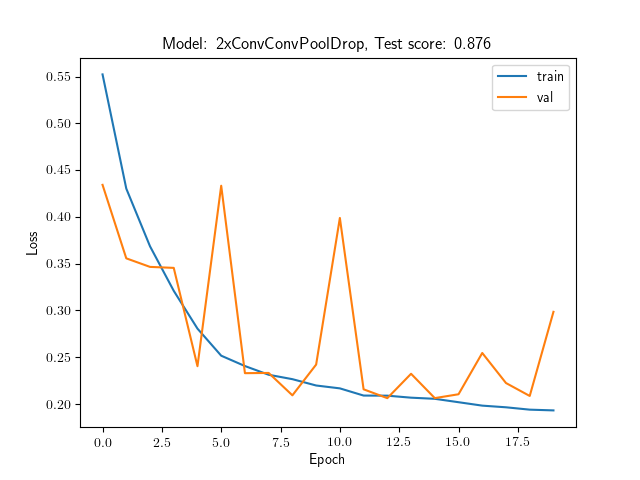
\includegraphics[width=200px]{../Plots/TrainTestScores/V0_L7_M500_N5_2xConvConvPoolDrop.png}
	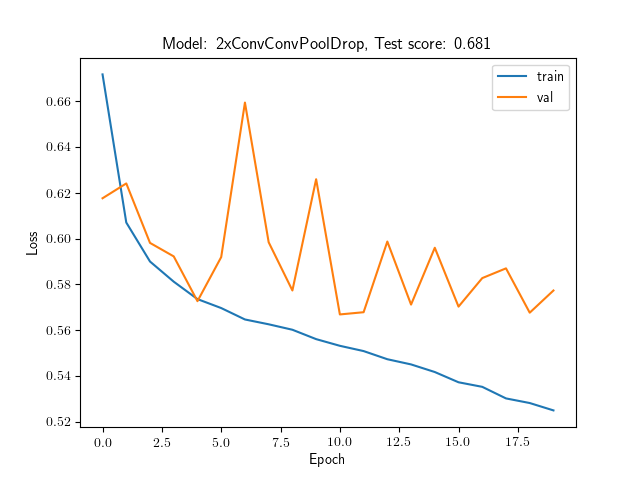
\includegraphics[width=200px]{../Plots/TrainTestScores/V1_L7_M500_N5_2xConvConvPoolDrop.png}
	\caption{Training history for (7, 500, 5) on the 2xConvConvPoolDrop architecture. \textbf{Left:} Training on raw spin configuration. \textbf{Right:} Training on vortex configuration. We see clearly that overfitting begins much earlier when we train on the vortex configuration, indicating sparseness of information in that dataset. Though regularization delays the onset of overfitting, we have not been able to increase the accuracy either by increasing dropout rate or the L$_2$-penalty. }
	\label{fig:train_val_history_cnn}
\end{figure}

Having finally obtained the (32, 1000, 1) dataset,\footnote{After 6x24 hours on my i7-7700k. Using CUDA would probably have sped this up quite significantly, but I wasn't aware of it at the time.} we briefly also present the corresponding results. First off, the heat capacity yields a critical temperature of
\begin{align}
T_\text{KT} = 1.16\ (03015075376883)
\end{align}
Due to an increased amount of data we expect better accuracy, but as the dataset has a class ratio of approximately 0.3 we anticipate issues related to that. As such, we attempted both SMOTEing and undersampling our dataset prior to training. It turns out, perhaps obviously, that SMOTE is not an appropriate algorithm for the system in question. As the resampled states are linear combinations of true states, the energy changes drastically. Training the nets on this highly biased dataset then leads to rather terrible predictions with $\Delta T_\text{KT} \approx 0.20$. On the other hand, we can still undersample. This moderately decreases the accuracy by approximately $0.05$ on average, but the most surprising thing is that we see no large gain in F1-scores. In fact, dropping any kind of resampling altogether leads to the results shown in Table \ref{tab:cnn_scores_32}.

\begin{table}[H]
	\centering
	\begin{tabular}{l|l|l|l|l}
		Architecture & Accuracy & F1 & $T_\text{KT}$ & $|\Delta T_\text{KT}|$ \\
		\hline 
		3xConv2xDropDense & .9991 & .9984 & 1.16 ($\dots$) & 0  \\
		3xConvPoolDrop & .9646 & .9398 & 1.16 (4824120603015) & 4.5$\cdot 10^{-3}$  \\
		2xConvPoolDrop & .9947 & .9910 & 1.16 (4824120603015) &  4.5$\cdot 10^{-3}$ \\
		2xConvConvPoolDrop & .9991 & .9984 & 1.16 ($\dots$) & 0 \\
		\hline
		nnsimple & .9223 & .8441 & 1.16 (4824120603015) & $4.5\cdot 10^{-3}$\\
		nnsimpler & .9734 & .9517 & 1.16 ($\dots$) & 0 \\
		nndeep & .8156 & .8301 & 1.16 ($\dots$) & 0
	\end{tabular}
	\caption{Scores for our nets trained on (32, 1000, 1), no resampling strategy was used. Regardless of class imbalance the F1-scores are still very high, indicating that the nets avoid the tendency to simply guess the majority class. When $\Delta T_\text{KT}$ is given as zero, it is so to numerical precision. Using 64-bit floats this corresponds to an error less than $10^{-16}$. It is quite puzzling that the models with $|\Delta T_\text{KT}| > 0$ predict the exact same $T_\text{KT}$ up to $10^{-16}$, even though their accuracies vary by up to 20\%. Performancewise all nets except 3xConv2xDropDense take a few minutes to train; the aforementioned net takes around two hours. As it performs identically to 2xConvConvPoolDrop, the choice for future training is clear.}
	\label{tab:cnn_scores_32}
\end{table}

Summing up the results, we again see the CNNs outperforming the NNs - at least for classification. When it comes to predicting $T_\text{KT}$, they both obtain the same value as found by Monte-Carlo simulations, up to $10^{-16}$. This is a little surprising when it comes to the NNs, especially the one with an accuracy of .8156. Looking at the prediction plot(see /Plots/Predictions/ on GitHub),\footnote{Note also that these plots show probability as a function of energy, whereas states are labeled by the temperature they were sampled at. Thus the probabilities will show the same fluctuations as the energy fluctuations occuring at any given temperature - assuming a good classifier. }  it is clear that the network is uncertain about most states, and hasn't learned very well. As such we attribute this success more to the law of large numbers and statistics than a success of the network itself - though obviously it wouldn't be possible if it had learned nothing at all. 

We do not present the results for (32, 1000, 1) trained on the vortex representation. As was the case for (7, 500, 5), classification accuracy takes a nosedive and is typically somewhere around 0.70. Quite simply, our results indicate that this type of feature engineering is not useful. This is however at odds with the results found in ref. \cite{PhysRevB.97.045207}, where they find that the vortex representation also yields high classification accuracy. Though they also find that accuracy increases with system size, it still cannot account for the abysmal performance of our nets trained on vortices. At the moment it is not clear to me where my error lies. The most likely candidate is the dataset itself. We already know that it does not correctly reproduce the transition temperature - it is possible that it also fails to properly capture the topological nature of the transition. This would explain the abysmal vortex training performance, and also indicates that our nets trained on the raw spin configurations are learning some other bulk feature - like magnetization - to classify states.


As for the ResNets, we can present no good results. There are a few reasons for this. One is that training a full ResNet is not feasible given my computing power, so our only choice is to use transfer learning. We did this with a ResNet pre-trained on ImageNet and with the last two residual blocks unlocked, obtaining accuracies of 0.49 and 0.72 with and without undersampling respectively. Note that due to class imbalance in (32, 1000, 1), only the score of 0.49 is indicative of how the ResNet performs. In fact its knowledge is of no use, and the topmost layers learn nothing at all. After 20 epochs it is still outputting only a single class. 

This is perhaps not too surprising. The ResNets are after all trained to recognize cats, boats and swords, so it is to be expected that they will have a hard time telling whether a state in the XY model is above or below the critical temperature. As such they may need to be fully trained on XY states if we are to see any performance increase over the other CNNs we have used. To be fair, we did not anticipate the extreme accuracy they achieved on e.g. (32, 1000, 1) - given that they perform so well, there is honestly little incentive to spend a week or two training a ResNet.


\section{Conclusion}
We have seen that both convolutional nets and regular neural nets are able to classify the states of the XY-model with extreme accuracy. Our best CNNs only misclassified 9 states on a test set containing 10 000 states, and predicted the critical temperature to a precision of $10^{-16}$. When it comes to classification, it is clear that CNNs outperform NNs no matter the size of the training set. The difference is however much smaller on (32, 1000, 1) than it is on (7, 500, 5). 

We have also seen that an extremely high classification accuracy is not needed to predict $T_\text{KT}$ to high precision - the best example of this being the regular neural net 'nndeep' predicting $T_\text{KT}$ to one part in $10^{-16}$ albeit only with a classification accuracy of 0.8156. This is likely the case because $T_\text{KT}$ is extracted through an averaging procedure which in a sense cancels out the noise of the bad predictions. This is an attractive feature for future projects; computational time is a constant annoyance, and if one can get away with training simple nets that is a nice advantage.

We also found that feature engineering by transforming to the vortex representation was detrimental, though it is likely that this is due to a fault either in my code or in the generated datasets. The ResNets were a colossal failure, but one that I should have anticipated. 

As for the future, I hope to be able to train nets that are able to classify vortex states in superfluids. To be fair, the current project has shown that the most difficult part is actually generating the datasets themselves. I would have liked to obtain $T_\text{KT}^\infty$; more computational power and/or some optimization would probably have done the job. The vortex representation was a failure for now, but it is one that I hope to resolve moving forward. Lastly, it would be quite interesting to plot the feature maps of the CNNs.


\bibliographystyle{unsrt}
\bibliography{bib}

\end{document}